\chapter*{Annexe 1}
\addcontentsline{toc}{chapter}{Annexe 1}
\newtheorem{kkk}{Théorème}
\newtheorem{li}{Lemme}

%changer le format des sections, subsections pour apparaittre sans le num de chapitre
\makeatletter
\renewcommand{\thesection}{\@arabic\c@section}
\makeatother

%recommencer la numérotation des section à "1"
\setcounter{section}{0}
Les théorèmes présentés dans cette annexe servent à démontrer d'autres théorèmes dans les chapitres précedents; l'axiome du choix va nous servir à démontrer le paradoxe de Hausdorff, et le théorème de Wallace-Bolyai-Gerwien à démontrer le théorème de Banach-Schröder-Bernstein.
\begin{kkk}(Axiome du choix)\cite{cite5}
  \hfill

\noindent
  Pour tout ensemble $X$ d'ensembles non vides, il existe une fonction définie sur $X$, appelée fonction de choix, qui à chaque ensemble $A$ appartenant à $X$ associe un élément de cet ensemble.
  \label{axiome}
\end{kkk}

\begin{kkk}(Théorème de Wallace-Bolyai-Gerwien)\label{wbg}\cite{cite6}
  \hfill

\noindent
Pour que deux polygones du plan aient la même aire, il faut et il suffit qu'ils soient équivalents par découpage fini.
\end{kkk}
\noindent
La condition nécessaire découle du \hyperref[pr]{Théorème 1 de la partie 3.3}, on va proposer une démonstration algorithmique de l'implication directe, on a tout d'abord besoin de quelques lemmes
\begin{li}
Tout polygone peut être scindé en un nombre fini de triangles.
\end{li}
\begin{proof}
  \hfill

  \noindent
  On va procéder par récurrence sur le nombre de sommets du polygone. Pour un polygone à trois sommets c'est évident parce qu'il est déjà un triangle. Soit $n\ge 3$ et on suppose que tout polygone à $k$ sommets avec $ 3 \le k \le n$ peut être scindé en un nombre fini de triangles.
  Considérons un polygone à $n+1$ sommets, et prenons le sommet le plus à gauche du polygone, ($P_3$ sur la figure suivante), et le segment formé des deux sommets voisins ($P_2$ et $P_4$ sur la figure suivante), si ce dernier est inclu dans le polygone alors Le triangle formé par ces trois sommets ($P_2P_3P_4$ sur la figure suivante) peut être ajouté à la liste des triangles qui composent le polygone. Le sommet ($P_3$ sur la figure suivante) est enlevé du polygone, et on applique récursivement la triangulation au polygone restant ($P_0P_1P_2P_4P_5P_6$ sur la figure suivante).
  \begin{figure}[h]
      \centering
      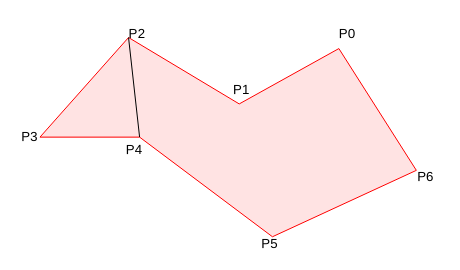
\includegraphics[scale=0.6]{images/x5.png}

      % \caption{Une représentation graphique d'un groupe libre de rang 2}
  \end{figure}

\noindent
sinon si le segment formé des deux sommets voisins n'est pas inclu dans polygone, il existe nécessairement un ou plusieurs sommets à
l'intérieur du triangle formé par ces sommets ($P_2P_3P_4$ sur la figure suivante) puisque ce segment va couper nécessairement l'intérieur d'un autre segment $[P_kP_l]$ et donc le somment le plus à gauche entre $P_k$ et $P_l$ va être à l'intérieur du triangle. Soit $P_j$ le sommet situé dans le triangle $P_2P_3P_4$ le plus loin de $P_2P_4$. Le segment $P_3P_j$ est à l'intérieur du polygone, car si un côté coupait ce segment, il aurait une extrémité dans le triangle $P_2P_3P_4$, plus éloigné de $P_2P_4$ que $P_j$.
% \newpage
La diagonale $P_3P_j$ permet de diviser le polygone initial en deux polygones le premier contien $P_3$, $P_2$ et $P_j$ et le deuxième contient $P_3$, $P_4$ et $P_j$ donc les deux polygones obtenus ont un nombre de sommets $\le n$. On applique récursivement la triangulation à ces deux polygones.

  \begin{figure}[h]
      \centering
      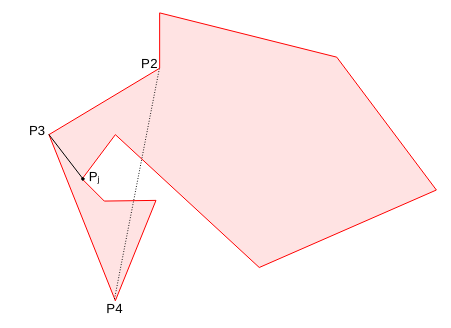
\includegraphics[scale=0.6]{images/x6.png}

      % \caption{Une représentation graphique d'un groupe libre de rang 2}
  \end{figure}
\end{proof}
\begin{li}
  Tout triangle peut être décomposé en un nombre fini de parties pour former un rectangle.
\end{li}
\begin{proof}
  \hfill

  \noindent
  Soit $ABC$ un triangle, et supposons que la droite passante par $B$ et perpendiculaire à la droite $(AC)$ coupe cette dernière en un point intérieur au segment $[AC]$ (on peut toujours trouver un tel B puisque il suffit de prendre le sommet du plus grand angle du triangle). Soit donc $D$ le milieu du segment $[AB]$, et soit $E$ l'intersection de la droite passante par $D$ et parallèle à $(AC)$, et soit $F$ la projection de $B$ sur $(DE)$.

  \begin{figure}[h]
          \centering
          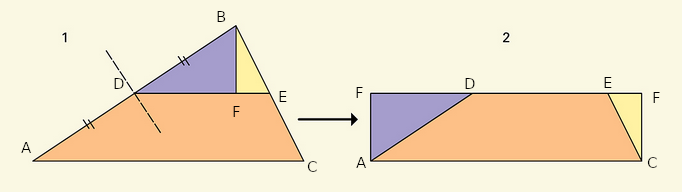
\includegraphics[scale=0.6]{images/xx1.png}

          % \caption{Une représentation graphique d'un groupe libre de rang 2}
      \end{figure}
\noindent
  Pour faire la décomposition ci-dessus il faut que  $BE = EC$, et $DE+DF+FE=2DE = AC$, et ceci est une conséquence directe de théorème de Thalès.

\end{proof}
\begin{li}
  Tout rectangle peut être transformé en un autre dont la longueur est inférieur à quatre fois sa largeur.
\end{li}
\newpage
\begin{proof}
  \hfill

  \noindent
  Si le rectangle a une longueur supérieur à quatre fois sa largeur on le découpe en deux (en longueur) et on le réarange de la manière suivante
  %
      \begin{figure}[h]
          \centering
          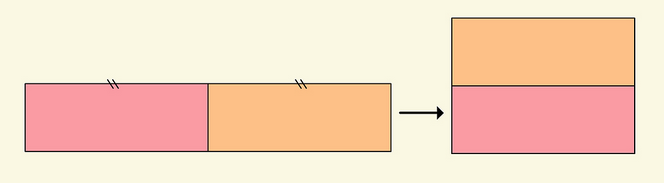
\includegraphics[scale=0.6]{images/x2.png}

          % \caption{Une représentation graphique d'un groupe libre de rang 2}
      \end{figure}

  \noindent
  et on répète cette opération jusqu'à obtenir un rectangle dont la longueur est inférieur à quatre fois sa largeur.
\end{proof}
\begin{li}
  Tout rectangle dont la longueur est inférieur à quatre fois sa largeur peut être décomposé en un caré.
\end{li}
\begin{proof}
Soit $ABCD$ un rectangle et soient $a=BC$ et $b=AB$ tel que $a<b$ (si $a=b$ alors il est déjà un caré), et soit $E$ le point du segment $[AB]$ tel que $AE = b-\sqrt{ab}$, et soit $F$ le point du segment $[CD]$ tel que $DF = \sqrt{ab}$, la perpendiculaire à $(CD)$ coupe $[CE]$ en $F$ si et seulement si $\sqrt{ab} \ge b-\sqrt{ab}$ c'est à dire si et seulement si $b \le 4a$, soit $G$ cette intersection.
\begin{figure}[h]
    \centering
    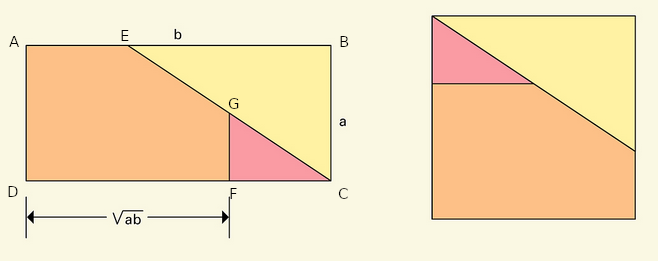
\includegraphics[scale=0.6]{images/xx3.png}

    % \caption{Une représentation graphique d'un groupe libre de rang 2}
\end{figure}

Pour pouvoir faire la décomposition ci-dessus, il faut que $FG +AD = \sqrt{ab}$. D'après le théorème de Thalès, $\frac{FG}{BC} = \frac{FC}{EB}$
c.à.d $FG = BC\frac{FC}{EB} = \frac{a(b-\sqrt{ab})}{\sqrt{ab}}$, et donc $FG +AD= FG + BC = \frac{a(b-\sqrt{ab})}{\sqrt{ab}} +a = \sqrt{ab}$
\end{proof}
\begin{li}
  Deux carrés peuvent être décomposés en un seul carré.
\end{li}
\begin{proof}
  \hfill

  \noindent
  Soit $ABCD$ et $EFGH$ deux carrés, et on suppose que la surface de $EFGH$ est inférieur à celle de $ABCD$. Posons le caré $EFGH$ à coté de $ABCD$ de sorte que $C=E$.
  \newpage
  \begin{figure}[h]
      \centering
      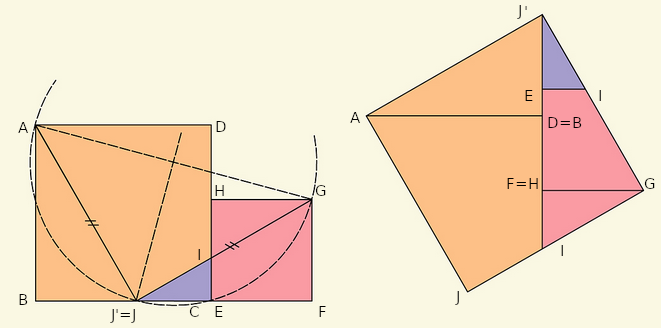
\includegraphics[scale=0.6]{images/xx4.png}

      % \caption{Une représentation graphique d'un groupe libre de rang 2}
  \end{figure}

\noindent
Soit $J=J'$ le point de $[BC]$ tel que $AJG$ est un triangle rectangle isocèle. On colle le triangle $ABJ'$ avec le polygone $AJGHD$ de sorte que $[AD] = [AB]$, on obtient donc un polygone  $AJGHJ'$ dont les coté $AJ$, $AJ'$ et $GJ$ sont égaux et les angles $\widehat{J'AJ}$ et $\widehat{AJG}$ sont droits, donc il suffit de montrer que les triangles $J'HG$ et $GJF$ sont égaux; c'est à dire il suffit de montrer que $HG=FG$ et $J'H=JF$, puisque $\widehat{J'HG} =\widehat{JFG}=90$. La première est évidente puisque $EFGH$ est un caré, et on a $J'H=JB+DH=AB-JE+AB-EF = 2AB-JF = JF$, puisque les triangles $ABJ$ et $JGF$ sont égaux car ils ont 2 angles égaux et un coté en commun.

\end{proof}
\begin{proof}[Démonstration du Théorème de Wallace-Bolyai-Gerwien]
  \hfill
  \begin{itemize}
    \item On décompose le premier polygone en un nombre fini de triangles.
    \item On transforme chaque triangle en un rectangle dont la longueur est inférieur à 4 fois la largeur.
    \item On transforme chaque rectangle en un carré.
    \item On fusionne les carrés, deux par deux, progressivement, jusqu'à avoir un unique grand carré.
    \item On refait la même chose pour le deuxième polygone et on superpose les découpages intervenus pour transformer le polygone 1 en carré à ceux obtenus pour transformer le polygone 2 en carré. Par construction, les pièces résultantes permettent de reconstituer le polygone 1 et le polygone 2.


  \end{itemize}
\end{proof}
% \begin{proof}
%   \hfill
%   \begin{itemize}
%     \item On commence par découper le premier polygone en triangles. Considérons le sommet le plus à gauche du polygone, $P_3$ sur la figure suivante, et le segment formé des deux sommets voisins $P_2$ et $P_4$, si ce dernier est inclu dans le polygone alors Le triangle $P_2P_3P_4$ peut être ajouté à la liste des triangles qui composent le polygone. Le sommet $P_3$ est enlevé du polygone, et on applique récursivement la triangulation au polygone restant $P_0P_1P_2P_4P_5P_6$.
%     \begin{figure}[h]
%         \centering
%         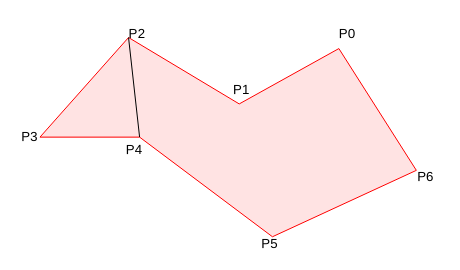
\includegraphics[scale=0.6]{images/x5.png}
%
%         % \caption{Une représentation graphique d'un groupe libre de rang 2}
%     \end{figure}
%
%     sinon si le segment formé des deux sommets voisins n'est pas à l'intérieur du polygone, il existe nécessairement un ou plusieurs sommets à
% l'intérieur du triangle $P_2P_3P_4$. Soit $P_j$ le sommet situé dans le triangle $P_2P_3P_4$ le plus loin de $P_2P_4$. Le segment $P_3P_j$ est à l'intérieur du polygone, car si un côté coupait ce segment, il aurait une extrémité dans le triangle $P_2P_3P_4$, plus éloigné de $P_2P_4$ que $P_j$.\\ La diagonale $P_3P_j$ permet de diviser le polygone initial en deux polygones. On applique récursivement la diagonalisation à ces deux polygones.
%
%     \begin{figure}[h]
%         \centering
%         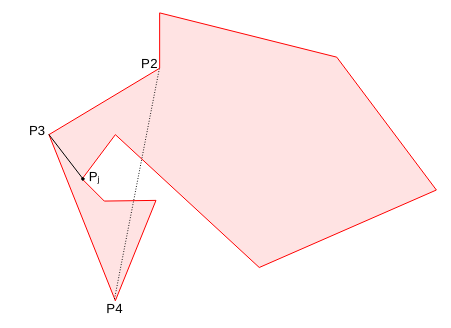
\includegraphics[scale=0.6]{images/x6.png}
%
%         % \caption{Une représentation graphique d'un groupe libre de rang 2}
%     \end{figure}
%     \newpage
%     \item Après, on transforme chaque triangle en un rectangle (ce découpage s'applique à tout triangle, car dans tout triangle au moins l'une des hauteurs coupe le côté opposé)
%     \begin{figure}[h]
%         \centering
%         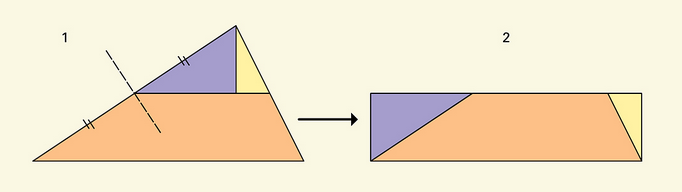
\includegraphics[scale=0.6]{images/x1.png}
%
%         % \caption{Une représentation graphique d'un groupe libre de rang 2}
%     \end{figure}
%     \item Si le rectangle a une longueur supérieur à quatre fois sa largeur on le découpe en deux (en longueur) et on le réarange de la manière suivante
%
%     \begin{figure}[h]
%         \centering
%         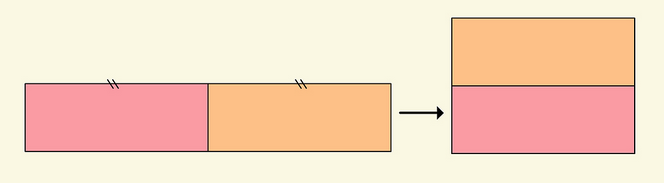
\includegraphics[scale=0.6]{images/x2.png}
%
%         % \caption{Une représentation graphique d'un groupe libre de rang 2}
%     \end{figure}
%
%     et on répète cette opération jusqu'à obtenir un rectangle dont la longueur est inférieur à quatre fois sa largeur.
%     \item On transforme chaque rectangle en carré de la manière suivante
%     \newpage
%
%     \begin{figure}[h]
%         \centering
%         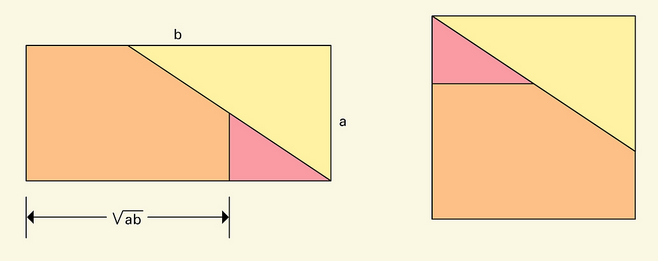
\includegraphics[scale=0.6]{images/x3.png}
%
%         % \caption{Une représentation graphique d'un groupe libre de rang 2}
%     \end{figure}
%
%     ceci est possible si et seulement si $\sqrt{ab} \ge b-\sqrt{ab}$ c'est à dire si et seulement si $b \le 4a$.
%     \item On fusionne les carrés, deux par deux, progressivement, jusqu'à avoir un unique grand carré de la manière suivante
%     \begin{figure}[h]
%         \centering
%         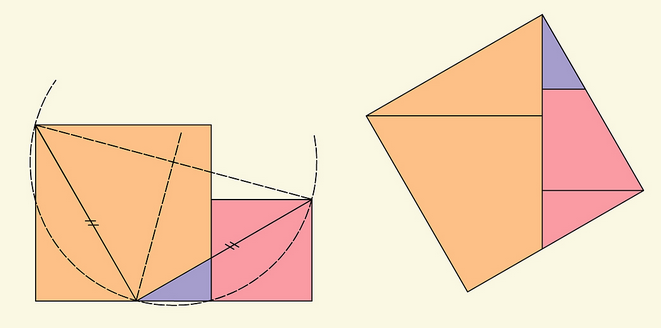
\includegraphics[scale=0.6]{images/x4.png}
%
%         % \caption{Une représentation graphique d'un groupe libre de rang 2}
%     \end{figure}
%     \item On refait la même chose pour le deuxième polygone et on superpose les découpages intervenus pour transformer le polygone 1 en carré à ceux obtenus pour transformer le polygone 2 en carré. Par construction, les pièces résultantes permettent de reconstituer le polygone 1 et le polygone 2.
%   \end{itemize}
%
% \end{proof}
